\documentclass{beamer}

% ---------- Theme & Packages ----------
\usetheme{Madrid}
\usecolortheme{seahorse}
\usepackage{amsmath, amssymb}
\usepackage{tikz}
\usetikzlibrary{positioning}

\title[Set Theory]{Set Theory: Fundamentals and Applications}
\subtitle{Sets, Operations, Inclusion--Exclusion \& Hasse Diagrams}
\author{Ahmed Sultan P}
\institute{IMSc 24}
\date{\today}

\begin{document}

% ---------- Title ----------
\begin{frame}
  \titlepage
\end{frame}

% ---------- Outline ----------
\begin{frame}{Outline}
  \tableofcontents
\end{frame}

% ============================================================
\section{Sets}
% ============================================================
\begin{frame}{What is a Set?}
  \begin{block}{Definition}
    A \textbf{set} is a well-defined collection of distinct objects,
    called \emph{elements} or \emph{members} of the set.
  \end{block}
  \pause
  \begin{itemize}
    \item Sets are usually denoted by capital letters: $A, B, C, \dots$
    \item Elements are denoted by lowercase letters: $a, b, c, \dots$
    \item If $x$ is an element of $A$, we write $x \in A$.
    \item If $x$ is not an element of $A$, we write $x \notin A$.
  \end{itemize}
  \pause
  \begin{exampleblock}{Examples}
    \begin{itemize}
      \item $V = \{a, e, i, o, u\}$ --- vowels of the English alphabet
      \item $\mathbb{N} = \{1, 2, 3, \dots\}$ --- natural numbers
      \item $E = \{2, 4, 6, 8, \dots\}$ --- even natural numbers
    \end{itemize}
  \end{exampleblock}
\end{frame}

\begin{frame}{Representation of Sets}
  Two common ways to represent a set:
  \begin{enumerate}
    \item \textbf{Roster (Tabular) Form:} List all elements, separated
          by commas, inside braces.
          \[
            A = \{1, 2, 3, 4, 5\}
          \]
    \item \textbf{Set Builder Form:} Describe elements by a common
          property (next section).
  \end{enumerate}
  \pause
  \begin{alertblock}{Note}
    \begin{itemize}
      \item Order of elements does not matter: $\{1,2,3\} = \{3,1,2\}$
      \item Repetition is ignored: $\{1,1,2\} = \{1,2\}$
    \end{itemize}
  \end{alertblock}
\end{frame}

% ============================================================
\section{Set Builder Form}
% ============================================================
\begin{frame}{Set Builder Form}
  \begin{block}{Definition}
    In \textbf{set builder form}, a set is described by stating a
    property $P(x)$ that its elements satisfy:
    \[
      A = \{\, x \mid P(x) \,\} \quad \text{or} \quad
      A = \{\, x : P(x) \,\}
    \]
    read as ``the set of all $x$ such that $P(x)$ holds.''
  \end{block}
  \pause
  \begin{exampleblock}{Examples}
    \begin{itemize}
      \item $A = \{\, x \mid x \in \mathbb{N},\ x \le 5 \,\}
            = \{1,2,3,4,5\}$
      \item $B = \{\, x \mid x \text{ is a vowel of the English alphabet}\,\}
            = \{a,e,i,o,u\}$
      \item $C = \{\, x \in \mathbb{Z} \mid x^2 = 4 \,\} = \{-2, 2\}$
      \item $D = \{\, 2n \mid n \in \mathbb{N} \,\} = \{2,4,6,\dots\}$
    \end{itemize}
  \end{exampleblock}
\end{frame}

\begin{frame}{Roster Form vs.\ Set Builder Form}
  \begin{center}
    \begin{tabular}{p{4.2cm} p{5.6cm}}
      \hline
      \textbf{Roster Form} & \textbf{Set Builder Form} \\ \hline
      $\{1, 4, 9, 16, 25\}$ &
        $\{\, x^2 \mid x \in \mathbb{N},\ x \le 5 \,\}$ \\[4pt]
      $\{2, 3, 5, 7, 11, 13\}$ &
        $\{\, x \mid x \text{ is a prime},\ x < 15 \,\}$ \\[4pt]
      $\{\dots,-2,-1,0,1,2,\dots\}$ &
        $\{\, x \mid x \in \mathbb{Z} \,\}$ \\ \hline
    \end{tabular}
  \end{center}
  \pause
  \begin{itemize}
    \item Set builder form is essential for \emph{infinite} sets or sets
          whose elements are inconvenient to list.
    \item Roster form is convenient for small, finite sets.
  \end{itemize}
\end{frame}

% ============================================================
\section{Types of Sets}
% ============================================================
\begin{frame}{Types of Sets (I)}
  \begin{description}
    \item[Empty (Null) Set] A set with no elements; denoted
      $\varnothing$ or $\{\}$.
      \\ Example: $\{x \in \mathbb{N} \mid x < 0\} = \varnothing$
    \pause
    \item[Singleton Set] A set with exactly one element.
      \\ Example: $\{0\}$
    \pause
    \item[Finite Set] A set with a finite number of elements.
      \\ Example: $\{1,2,3\}$; cardinality $|A| = 3$
    \pause
    \item[Infinite Set] A set that is not finite.
      \\ Example: $\mathbb{N}, \mathbb{Z}, \mathbb{R}$
  \end{description}
\end{frame}

\begin{frame}{Types of Sets (II)}
  \begin{description}
    \item[Equal Sets] $A = B$ iff they have exactly the same elements.
      \\ Example: $\{1,2\} = \{2,1\}$
    \pause
    \item[Equivalent Sets] $A \sim B$ iff $|A| = |B|$.
      \\ Example: $\{1,2,3\} \sim \{a,b,c\}$
    \pause
    \item[Subset] $A \subseteq B$ iff every element of $A$ is in $B$.
      \\ \textbf{Proper subset:} $A \subset B$ iff $A \subseteq B$ and
      $A \ne B$.
    \pause
    \item[Power Set] $\mathcal{P}(A)$: the set of all subsets of $A$.
      \\ If $|A| = n$, then $|\mathcal{P}(A)| = 2^n$.
      \\ Example: $\mathcal{P}(\{1,2\}) =
         \{\varnothing, \{1\}, \{2\}, \{1,2\}\}$
    \pause
    \item[Universal Set] The set $U$ containing all objects under
      discussion.
    \pause
    \item[Disjoint Sets] $A$ and $B$ are disjoint iff
      $A \cap B = \varnothing$.
  \end{description}
\end{frame}

% ============================================================
\section{Set Operations}
% ============================================================
\begin{frame}{Set Operations}
  Let $A$ and $B$ be subsets of a universal set $U$.
  \begin{description}
    \item[Union] $A \cup B = \{\, x \mid x \in A \text{ or } x \in B \,\}$
    \item[Intersection] $A \cap B = \{\, x \mid x \in A \text{ and } x \in B \,\}$
    \item[Difference] $A - B = \{\, x \mid x \in A \text{ and } x \notin B \,\}$
    \item[Complement] $A' = \overline{A} = \{\, x \in U \mid x \notin A \,\}$
    \item[Symmetric Difference]
      $A \,\triangle\, B = (A - B) \cup (B - A)$
  \end{description}
  \pause
  \begin{exampleblock}{Example: $A=\{1,2,3,4\}$, $B=\{3,4,5,6\}$, $U=\{1,\dots,8\}$}
    $A \cup B = \{1,2,3,4,5,6\}$,\quad
    $A \cap B = \{3,4\}$,\\
    $A - B = \{1,2\}$,\quad
    $A' = \{5,6,7,8\}$,\quad
    $A \triangle B = \{1,2,5,6\}$
  \end{exampleblock}
\end{frame}

\begin{frame}{Venn Diagrams of Basic Operations}
  \begin{center}
  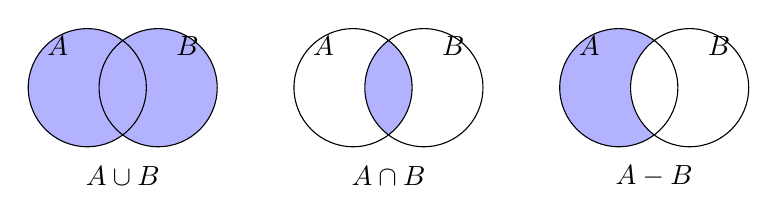
\begin{tikzpicture}[scale=0.75]
    % ---- Union ----
    \begin{scope}
      \fill[blue!30] (0,0) circle (1) (1.2,0) circle (1);
      \draw (0,0) circle (1) (1.2,0) circle (1);
      \node at (0.6,-1.5) {$A \cup B$};
      \node at (-0.5,0.7) {$A$};
      \node at (1.7,0.7) {$B$};
    \end{scope}
    % ---- Intersection ----
    \begin{scope}[xshift=4.5cm]
      \begin{scope}
        \clip (0,0) circle (1);
        \fill[blue!30] (1.2,0) circle (1);
      \end{scope}
      \draw (0,0) circle (1) (1.2,0) circle (1);
      \node at (0.6,-1.5) {$A \cap B$};
      \node at (-0.5,0.7) {$A$};
      \node at (1.7,0.7) {$B$};
    \end{scope}
    % ---- Difference ----
    \begin{scope}[xshift=9cm]
      \fill[blue!30] (0,0) circle (1);
      \begin{scope}
        \clip (0,0) circle (1);
        \fill[white] (1.2,0) circle (1);
      \end{scope}
      \draw (0,0) circle (1) (1.2,0) circle (1);
      \node at (0.6,-1.5) {$A - B$};
      \node at (-0.5,0.7) {$A$};
      \node at (1.7,0.7) {$B$};
    \end{scope}
  \end{tikzpicture}
  \end{center}
  \pause
  \begin{center}
  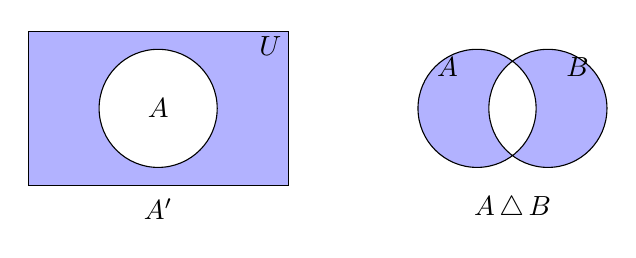
\begin{tikzpicture}[scale=0.75]
    % ---- Complement ----
    \begin{scope}
      \fill[blue!30] (-1.6,-1.3) rectangle (2.8,1.3);
      \fill[white] (0.6,0) circle (1);
      \draw (-1.6,-1.3) rectangle (2.8,1.3);
      \draw (0.6,0) circle (1);
      \node at (0.6,-1.7) {$A'$};
      \node at (0.6,0) {$A$};
      \node at (2.5,1.05) {$U$};
    \end{scope}
    % ---- Symmetric difference ----
    \begin{scope}[xshift=6cm]
      \fill[blue!30] (0,0) circle (1) (1.2,0) circle (1);
      \begin{scope}
        \clip (0,0) circle (1);
        \fill[white] (1.2,0) circle (1);
      \end{scope}
      \draw (0,0) circle (1) (1.2,0) circle (1);
      \node at (0.6,-1.7) {$A \,\triangle\, B$};
      \node at (-0.5,0.7) {$A$};
      \node at (1.7,0.7) {$B$};
    \end{scope}
  \end{tikzpicture}
  \end{center}
\end{frame}

\begin{frame}{Laws of Set Algebra}
  \small
  \begin{center}
    \begin{tabular}{l l}
      \hline
      \textbf{Law} & \textbf{Statement} \\ \hline
      Idempotent    & $A \cup A = A$, \quad $A \cap A = A$ \\
      Commutative   & $A \cup B = B \cup A$, \quad $A \cap B = B \cap A$ \\
      Associative   & $(A \cup B) \cup C = A \cup (B \cup C)$ \\
                    & $(A \cap B) \cap C = A \cap (B \cap C)$ \\
      Distributive  & $A \cup (B \cap C) = (A \cup B) \cap (A \cup C)$ \\
                    & $A \cap (B \cup C) = (A \cap B) \cup (A \cap C)$ \\
      Identity      & $A \cup \varnothing = A$, \quad $A \cap U = A$ \\
      Complement    & $A \cup A' = U$, \quad $A \cap A' = \varnothing$ \\
      De Morgan's   & $(A \cup B)' = A' \cap B'$ \\
                    & $(A \cap B)' = A' \cup B'$ \\ \hline
    \end{tabular}
  \end{center}
\end{frame}

% ============================================================
\section{Inclusion--Exclusion Principle}
% ============================================================
\begin{frame}{Inclusion--Exclusion Principle}
  \begin{block}{For two sets}
    \[
      |A \cup B| \;=\; |A| + |B| - |A \cap B|
    \]
  \end{block}
  \pause
  \begin{block}{For three sets}
    \begin{align*}
      |A \cup B \cup C| \;=\;& |A| + |B| + |C| \\
      &- |A \cap B| - |B \cap C| - |A \cap C| \\
      &+ |A \cap B \cap C|
    \end{align*}
  \end{block}
  \pause
  \textbf{Idea:} Adding $|A|$ and $|B|$ counts elements of
  $A \cap B$ \emph{twice}, so we subtract the overlap once.
\end{frame}

\begin{frame}{General Form and Example}
  \begin{block}{General form ($n$ sets)}
    \[
      \Bigl| \bigcup_{i=1}^{n} A_i \Bigr|
      = \sum_{i} |A_i|
      - \sum_{i<j} |A_i \cap A_j|
      + \sum_{i<j<k} |A_i \cap A_j \cap A_k|
      - \cdots
      + (-1)^{n+1} |A_1 \cap \cdots \cap A_n|
    \]
  \end{block}
  \pause
  \begin{exampleblock}{Example}
    In a class of 50 students, 30 study Mathematics, 25 study Physics,
    and 10 study both. How many study at least one subject?
    \[
      |M \cup P| = |M| + |P| - |M \cap P| = 30 + 25 - 10 = 45
    \]
    Students studying neither: $50 - 45 = 5$.
  \end{exampleblock}
\end{frame}

% ============================================================
\section{Hasse Diagrams}
% ============================================================
\begin{frame}{Partial Orders and Hasse Diagrams}
  \begin{block}{Partially Ordered Set (Poset)}
    A relation $\preceq$ on a set $S$ is a \textbf{partial order} if it
    is
    \begin{itemize}
      \item \textbf{Reflexive:} $a \preceq a$
      \item \textbf{Antisymmetric:} $a \preceq b$ and $b \preceq a$
            $\Rightarrow a = b$
      \item \textbf{Transitive:} $a \preceq b$ and $b \preceq c$
            $\Rightarrow a \preceq c$
    \end{itemize}
    The pair $(S, \preceq)$ is called a \emph{poset}.
  \end{block}
  \pause
  \begin{block}{Hasse Diagram}
    A simplified graph of a finite poset, obtained by:
    \begin{enumerate}
      \item Removing all self-loops (reflexivity is implicit).
      \item Removing edges implied by transitivity.
      \item Drawing $b$ \emph{above} $a$ whenever $a \prec b$
            (arrows omitted; direction is upward).
    \end{enumerate}
  \end{block}
\end{frame}

\begin{frame}{Example 1: Divisibility on $\{1,2,3,4,6,12\}$}
  Poset: $(\{1,2,3,4,6,12\}, \mid)$ where $a \mid b$ means
  ``$a$ divides $b$''.
  \begin{center}
    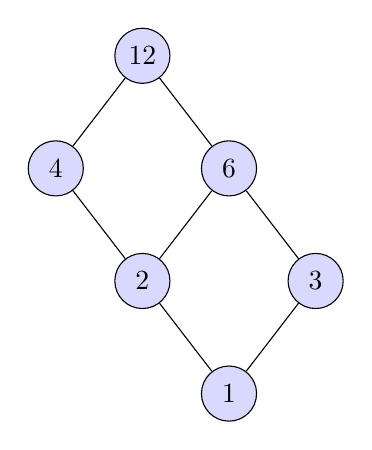
\begin{tikzpicture}[scale=1.1,
        every node/.style={circle, draw, fill=blue!15,
                           minimum size=7mm, inner sep=1pt}]
      \node (n1)  at (1, 0)   {$1$};
      \node (n2)  at (0, 1.3) {$2$};
      \node (n3)  at (2, 1.3) {$3$};
      \node (n4)  at (-1,2.6) {$4$};
      \node (n6)  at (1, 2.6) {$6$};
      \node (n12) at (0, 3.9) {$12$};
      \draw (n1) -- (n2);
      \draw (n1) -- (n3);
      \draw (n2) -- (n4);
      \draw (n2) -- (n6);
      \draw (n3) -- (n6);
      \draw (n4) -- (n12);
      \draw (n6) -- (n12);
    \end{tikzpicture}
  \end{center}
  \small Edge $1$--$4$ is omitted because $1 \mid 2$ and $2 \mid 4$
  (transitivity).
\end{frame}

\begin{frame}{Example 2: Power Set of $\{a,b,c\}$ under $\subseteq$}
  Poset: $(\mathcal{P}(\{a,b,c\}), \subseteq)$
  \begin{center}
    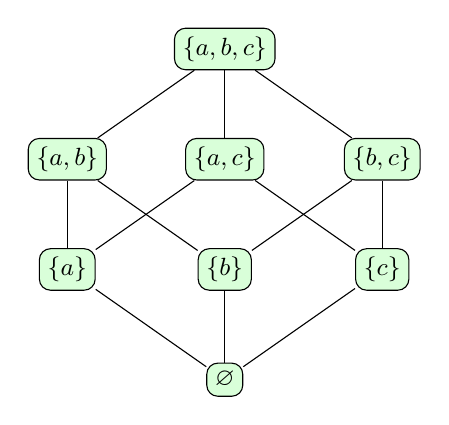
\begin{tikzpicture}[scale=1.0,
        every node/.style={draw, rounded corners, fill=green!15,
                           inner sep=3pt, font=\small}]
      \node (e)   at (0, 0)    {$\varnothing$};
      \node (a)   at (-2,1.4)  {$\{a\}$};
      \node (b)   at (0, 1.4)  {$\{b\}$};
      \node (c)   at (2, 1.4)  {$\{c\}$};
      \node (ab)  at (-2,2.8)  {$\{a,b\}$};
      \node (ac)  at (0, 2.8)  {$\{a,c\}$};
      \node (bc)  at (2, 2.8)  {$\{b,c\}$};
      \node (abc) at (0, 4.2)  {$\{a,b,c\}$};
      \draw (e)  -- (a);  \draw (e)  -- (b);  \draw (e)  -- (c);
      \draw (a)  -- (ab); \draw (a)  -- (ac);
      \draw (b)  -- (ab); \draw (b)  -- (bc);
      \draw (c)  -- (ac); \draw (c)  -- (bc);
      \draw (ab) -- (abc); \draw (ac) -- (abc); \draw (bc) -- (abc);
    \end{tikzpicture}
  \end{center}
\end{frame}

\begin{frame}{Reading a Hasse Diagram}
  \begin{itemize}
    \item \textbf{Maximal element:} no element lies above it.
    \item \textbf{Minimal element:} no element lies below it.
    \item \textbf{Greatest element:} above \emph{every} other element
          (if it exists).
    \item \textbf{Least element:} below \emph{every} other element
          (if it exists).
  \end{itemize}
  \pause
  \begin{exampleblock}{For $(\{1,2,3,4,6,12\}, \mid)$}
    \begin{itemize}
      \item Least element: $1$ \quad (divides everything)
      \item Greatest element: $12$ \quad (divisible by everything)
    \end{itemize}
  \end{exampleblock}
  \pause
  \begin{alertblock}{Remember}
    Comparability in a Hasse diagram means there is an \emph{upward
    path} between two elements --- not merely that one is drawn higher.
  \end{alertblock}
\end{frame}

% ---------- Summary ----------
\begin{frame}{Summary}
  \begin{itemize}
    \item A \textbf{set} is a well-defined collection of distinct
          objects; written in roster or \textbf{set builder} form.
    \item Key \textbf{types}: empty, singleton, finite/infinite,
          equal/equivalent, subsets, power set, universal, disjoint.
    \item \textbf{Operations}: union, intersection, difference,
          complement, symmetric difference --- governed by the laws of
          set algebra (incl.\ De Morgan's laws).
    \item \textbf{Inclusion--Exclusion} counts a union without
          double-counting overlaps.
    \item \textbf{Hasse diagrams} give a compact picture of finite
          posets by dropping reflexive and transitive edges.
  \end{itemize}
  \vfill
  \begin{center}
    \Large Thank you!
  \end{center}
\end{frame}

\end{document}
